\title{A short report on: \\Transcription Factor Activity of C. Elegans}
\author{
        Muhammad Arifur Rahman \\
        Department of Computer Science\\
        The University of Sheffield\\ Sheffield, UK\\
        %            \and
        %Department of Computer Science\\
        %Technion---Israel Institute of Technology\\
        %Technion City, Haifa 32000, \underline{Israel}
}
\date{\today}

\documentclass[12pt]{article}

\usepackage{graphicx} % Allows including images
\usepackage{booktabs} % Allows the use of \toprule, \midrule and \bottomrule in tables
\usepackage{epstopdf} % Allows to view .eps files
\usepackage{amsmath}
\usepackage{amssymb}
\usepackage{color}
\usepackage{url}

\begin{document}
\maketitle

%\begin{abstract}
%This is the paper's abstract \ldots
%\end{abstract}

\section{Motivation}
	\begin{itemize}
	  \item Caenorhabditis Elegans, a saprophytic nematode is an inhabitant of soil and leaf-litter and found 
		in most of the parts of the world~\cite{hope}.
	  \item Scientific reports on C.Elegans appeared in the literature for more than 100 years.
	  \item After the genetics paper of Brenner's ~\cite{brenner} C. Elegans emerged as an important experimental model.
	  \item Based on the bioinformatics approach used C. Elegans is 60-80\% homologies with human genes. ~\cite{kaletta}.
	  \item Within a very short period of time (approximately 3days) allows a large-scale (300+ of offspring) production ~\cite{hope}. 
	  \item In molecular biology and genetics, a transcription factor is a protein that binds to specific DNA sequence.
	  \item Transcription factors control the flow (or transcription) of genetic information from DNA to mRNA. 
	  \item To develop models of cellular processes quantitative estimation of the regulatory relationship between transcription factors and genes is a basic requirement. 
	  \item It is difficult for a number of reasons: transcription factors’ expression levels are often low and noisy, and many transcription factors are post- transcriptionally regulated. 
	  \item So, from the expression levels of their target genes it is functional to infer the activity of the transcription factors.

	\end{itemize}

\section{Mehhodology}\label{mehhodology}
To determine the gene specific transcription factor activity of C. Elegans we have followd Sanguinetti's probabilistic
dynamic model ~\cite{sanguinetti:01} for quantative inference.

	
\section{Data}\label{data}

We have collected the data from three different sources-
%A much longer \LaTeXe{} example was written by Gil~\cite{Gil:02}.
%A much smaller \LaTeXe{} example is using by by Arif~\cite{Arif:01}.
	
\paragraph{Expression level:}
The point estimate of the expression label and the uncertainty of the expression level were 
extracted from the micro array data provided by Prof. Andrew Cossins using the tool puma ~\cite{puma}.  


\paragraph{Transcription Factors:}
C.Elegans differential gene expression database (EDGEdb) ~\cite{edgedb:01} is the storage and retrieval 
of protein-DNA interactions. EDGEdb contains the sequence information of C.Elegans's 934 transcription
factor and their DNA binding domains. It also represents the protein-DNA interactions between transcription
and regulatory elements. At the initial point we have considered these 934 transcription factors for 
our experiment. 


\paragraph{Connectivity between Genes and Transcription Factors:}
WormNet ~\cite{wormnet:url} is a modified Bayesian integration based probabilistic functional gene network of C. Elegans.
Here the true functional linkage between genes was measured with its associated log-likelihood score.
WormNet also tried to figure out the known functionality of C.Elegans and the links between 
different types of data from different types of organisms ~\cite{wormnet:01, wormnet:02}.

Evidence code of ~\cite{wormnet:url} represent 21 different types of relations between genes.
Initially among these relations we choose Co-citation of worm gene (CE-CC), Co-expression among worm genes(CE-CX),
Co-citation of human genes (HS-CC) and Co-expression among human genes (HS-CX) to get the connectivity between genes 
and transcription factors. This relation leads to create a binary matrix of 0's and 1's. If there is any
evidence of connectivity between any gene to a given transcription factor, then the connectivity matrix
is indicated by 1. Otherwise, the value is 0. We need to know about the exact relation. 



\section{Results}\label{results}
In this section we describe the results.

Genes regulated by multiple TF
        \begin{table}
	  \begin{tabular}{l l }
	      \textbf{Gene Name} & \textbf{Regulators activity} \\
	      {\color{red}C44B12.5} & {\color{blue} Y116A8C.35 }= $ 1.719797 \pm 3.493205 $, \\ 
				    & {\color{blue}F33A8.3} = $ 1.415785 \pm 3.492985$ \\~\\

		{\color{red}Y105E8B.3} & {\color{blue} Y54G2A.1} = $ 0.07157665 \pm 1.2222137 $ \\
		  & {\color{blue} F33D11.12} = $ 0.03861905 \pm 0.7252534 $ \\
 		  & {\color{blue} ZK370.2} = $ -1.20157055 \pm  2.0318513 $\\~\\
		    
	      {\color{red} Y105E8B.3} & {\color{blue} T20B12.8 } = $ 0.25474933 \pm  2.5665869 $ \\
		  			& {\color{blue} F33A8.3 } = $ 0.11619828  \pm  3.5107742 $ \\
 		  			& {\color{blue} Y116A8C.35 } = $ 0.03289664 \pm  3.8071374 $ \\
					& {\color{blue} F11A10.2 } = $ 0.03016348 \pm 1.7737585 $ \\
 		  			& {\color{blue} C16A3.7  } = $ 0.01883489 \pm  $ 0.9431105\\

	  \end{tabular}
	  \caption{Genes regulated by multiple TF}
	  \end{table}


      %\begin{block}
      Gene Specific TFA of T20B12.8
    
      \begin{figure}[h]
      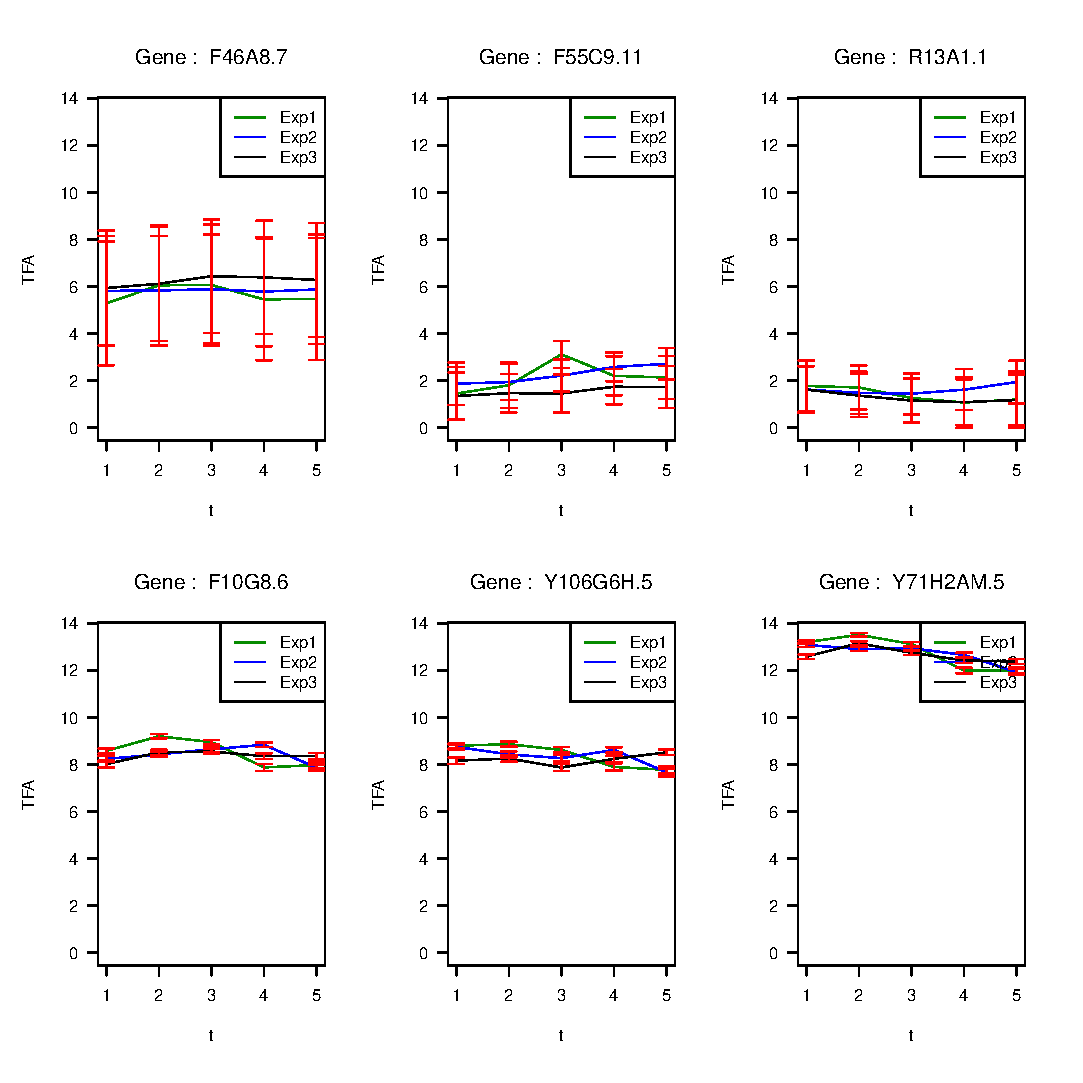
\includegraphics[width=1.0\linewidth]{picture/T20B12_8_3.eps}
      \caption{Gene Specific TFA of T20B12.8}
      \end{figure}

      %\end{block}

      
      %-- Block 3-3
      %--------------------------------------------------------------------------------------------
      %\begin{block
      Gene Specific TFA of ZK370.2
      
      \begin{figure}[h]
      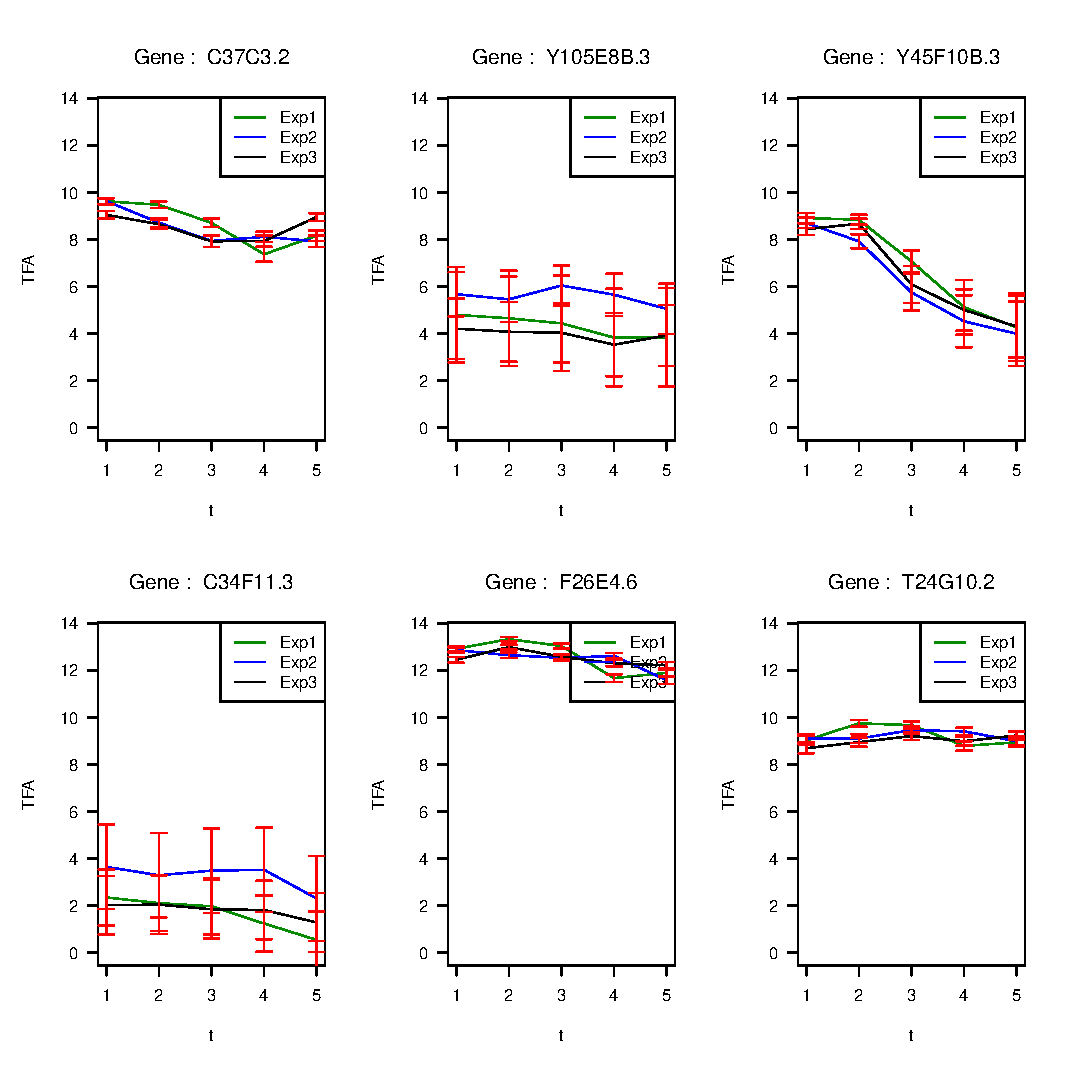
\includegraphics[width=1.0\linewidth]{picture/ZK370_2_3.eps}
      \caption{Gene Specific TFA of ZK370.2}
      \end{figure}

      %\end{block}


\section{Conclusions}\label{conclusions}
We with worked hard, and achieved very little. We worked hard, and achieved very little. We worked hard, and achieved very little.

\bibliographystyle{abbrv}
\bibliography{bib_chipDyno}

\end{document}
